\documentclass[12pt]{article}
\usepackage[top=3cm, bottom=2.5cm, left=2cm, right=2.5cm]{geometry}
\usepackage{listings}
\usepackage{float}
\usepackage{subfig}
\usepackage{graphicx}
\usepackage{booktabs}
\usepackage{ptext}
\usepackage{amsmath}
\usepackage[usenames,dvipsnames]{color,xcolor}
\usepackage{xepersian}
\setlatintextfont[Scale=1]{Times New Roman}
\settextfont[Scale=1]{XB Niloofar}

\title{تمرین تئوری سری اول مبانی یادگیری عمیق}
\author{کورش تقی پور پاسدار 
	\lr{400521207}}
\makeglossary
\begin{document}
	\maketitle
	\tableofcontents
	\section{سوال اول}
	\subsection{الف}
	
	\subsubsection{فرمول کلی}
	در لایه‌های کانولوشنی، تعداد پارامتر‌ها از فرمول زیر بدست می‌آید.
	\begin{eqnarray*}
		P &=& (Cin\times H\times W + 1)\times Cout 
	\end{eqnarray*}
	لایه‌های \lr{MaxPolling}, \lr{AvgPolling}, \lr{Dropout} پراامتری ندارند.
	تعداد پارامتر‌های لایه خطی هم از فرمول زیر بدست می‌آید.
	\begin{eqnarray*}
		P &=& (Nin + 1)\times Nout 
	\end{eqnarray*}
	که \lr{Nin} به تعداد ویژگی‌های ورودی و \lr{Nout} تعداد ویژگی‌های خروجی اشاره دارد.
	\subsubsection{\lr{Layer 1}}
	در این لایه اندازه خروجی برابر با $32\times128\times128$ می‌باشد. همچنین تعداد پارامترهای آن برابر با \lr{4736} می‌باشد.میدان تاثیر این لایه برابر با \lr{49} می‌باشد.
	\subsubsection{\lr{Layer 2}}
	در این لایه اندازه خروجی برابر با $64\times62\times62$ می‌باشد. تعداد پارامترهای آن نیز برابر با \lr{51264} می‌باشد. همچنین میدان تاثیر آن نیز برابر با \lr{1225} پیکسل از ابعاد تصویر ورودی می‌باشد.
	\subsubsection{\lr{Layer 3}}
	در این لایه، اندازه خروجی برابر با $64\times31\times31$ می‌باشد. این لایه پارامتری ندارد و میدان تاثیر لایه برابر با \lr{4900} پیکسل از تصویر ورودی می‌باشد.
	\subsubsection{\lr{Layer 4}}
	در این لایه، اندازه خروجی برابر با $128\times27\times27$ می‌باشد. این لایه \lr{73856} پارامتر دارد.
	\subsubsection{\lr{Layer 5}}
	در این لایه، اندازه خروجی برابر با $128\times25\times25$ می‌باشد. این لایه \lr{147584} پارامتر دارد.
	\subsubsection{\lr{Layer 6}}
	در این لایه، اندازه خروجی برابر با $128\times12\times12$ می‌باشد. این لایه پارامتری ندارد.
	\subsubsection{\lr{Layer 7}}
	در این لایه، اندازه خروجی برابر با $256\times10\times10$ می‌باشد. این لایه \lr{295168} پارامتر دارد.
	\subsubsection{\lr{Layer 8}}
	در این لایه، اندازه خروجی برابر با $256\times5\times5$ می‌باشد. این لایه پارامتری ندارد.
	\subsubsection{\lr{Layer 9}}
	در این لایه (فرض می‌شود یک لایه \lr{Flatten} قبل آن اعمال شده است) اندازه خروجی برابر با \lr{1024} بوده و تعداد پارامترهای آن \lr{6554624} می‌باشد. 
	\subsubsection{\lr{Layer 10}}
	در این لایه اندازه خروجی تغییری نکرده و پارامتری هم ندارد.
	\subsubsection{\lr{Layer 11}}
	در این لایه تعداد پارامترها برابر با \lr{10250} می‌باشد و اندازه خروجی هم برابر با \lr{10} می‌باشد.
	
	\section{سوال دوم}
	\subsection{الف}
	بایاس به طور خلاصه به میزان خطای ناشی از ساده‌سازی بیش از حد مدل و واریانس به حساسیت بیش از حد مدل به داده‌های آموزشی اشاره دارد. این دو مورد در تضاد با یکدیگر بوده و افزایش قدرت مدل به افزایش واریانس و کاهش بایاس منجر می‌شود و برعکس. در حالت‌هایی که مدل ساده بوده،‌مدل توانایی یادگیری کافی داده‌ها را ندارد. به همین دلیل در این حالت بایاس مدل زیاد بوده و واریانس آن کم می‌باشد. در حالتی که مدل پیچیده است، مدل می‌تواند داده‌ها را یادبگیرد و بایاس آن کم است، ولی ممکن است حساسیت بیش از حد به داده‌ها پیدا کند و واریانس آن زیاد شود. در تصویر زیر می‌توان به درک شماتیکی از این دو مفهوم رسید.
	\begin{figure}[H]
		\centering
		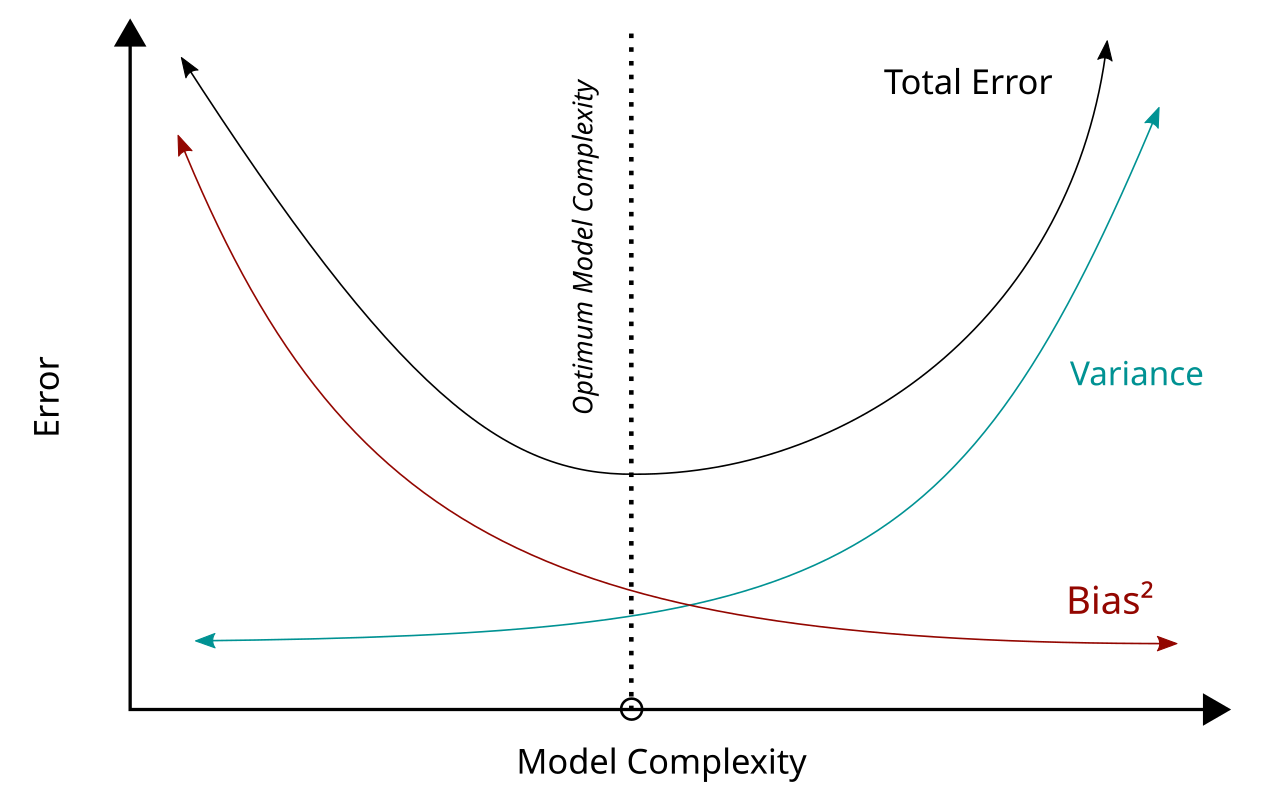
\includegraphics[scale=0.3]{pic_1}
		\caption{Bias-Variance Trade-off}
	\end{figure}
	\subsection{ب}
	درصورتی‌که عملکرد مدل عصبی برروی داده‌های آموزشی خوب باشد ولی برروی داده‌های تست پایین باشد، مدل عصبی دچار \lr{Overfitting} شده است. \lr{Overfitting} زمانی رخ می‌دهد که مدل بجای الگو‌های کلی بین داده‌ها، نویزها را نیز یاد بگیرد یا به عبارت دیگر، داده‌ها را حفظ کند. از راه‌کارهای مقابله با آن می‌توان به استفاده از \lr{dropout}، کاهش قدرت مدل عصبی یا کاهش تعداد \lr{epoch} ها اشاره کرد.
	\subsection{ج}
	مشکل ناپدید شدن گرادیان، به کاهش بسیار زیاد گرادیان به خصوص برای پارامترهای لایه‌های ابتدایی‌تر گفته می‌شود که سبب می‌شود تا بدلیل کاهش بسیار زیاد گرادیان محاسبه شده و نزدیک صفر بودن آن، پارامترهای آن لایه‌ها در عمل تغییر چندانی نکرده و آموزش نبینند. از طرفی، انفجار گرادیان به مقداردهی بسیار زیاد گرادیان گفته می‌شود که سبب می‌شود تا پارامتر مربوط به آن گرادیان به نقطه نامعلومی رفته و تابع مدل تغییر بسیار زیادی بکند. 
	\newline
	ناپدید شدن گرادیان عمدتا در توابع فعالسازی مانند \lr{Sigmoid} که مشتق آنها معمولا کوچک است رخ می‌دهد و زمانی که از این توابع در لایه‌های میانی استفاده کنیم که سبب می‌شود با ضرب چندباره گرادیان در این مقادیر، گرادیان بسیار کوچک شود.
	\newline
	انفجار گرادیان هم در توابعی مانند \lr{ReLU} رخ می‌دهد که خروجی آنها به یک بازه محدود نیست. 
	\subsection{د}
	عمیق‌تر کردن شبکه \lr{MLP} سبب می‌شود تا تعداد نورون‌های لازم به طور نمایی کاهش یابد. به عبارت دیگر، یک شبکه \lr{MLP} سطحی \LTRfootnote{Shallow} نسبت به یک شبکه عمیق \LTRfootnote{Deep} که هردو عملکرد مشابهی دارند، تعداد نورون‌های بیشتری (از مرتبه نمایی) دارد.
	\newline
	درمورد بررسی نتایج شبکه‌های عمیق و سطحی، باید گفت که درصورتی که در شبکه سطحی از نورون‌های کافی استفاده شود، می‌تواند همانند شبکه عمیق و یا حتی بهتر عمل کند. به عبارت دیگر، عمیق بودن شبکه لزوما به معنی کسب نتایج بهتر نیست. البته لازم به ذکر است که شبکه‌های عمیق به دلیل تعداد کمتر نورون‌ها،‌ نیاز به بهینه‌کردن نورون‌های کمتری بوده، در نتیجه آموزش سریعتر و در نتیجه همگرایی \LTRfootnote{Convergence} سریعتری دارند.
	\section{سوال سوم}
			با توجه به  عملیات کانولوشن، حاصل اعمال فیلتر برروی ورودی بصورت زیر خواهد بود.
		
		\begin{table}[h!]
			\centering
			\begin{tabular}{|c|c|}
				\toprule
				\lr{-18} & \lr{7} \\
				\midrule
				\lr{4} & \lr{10} \\
				\bottomrule
			\end{tabular}
		\end{table}
		حال با اعمال لایه ادغام حداکثر سراسری\LTRfootnote{\lr{Global max pooling(GAP)}}، خروجی برابر با \lr{10} خواهد شد. حال  خانه‌های خروجی را بصورت $z_{1}, z_{2}, z_{3}, z_{4}$ نمایش دهیم که به ترتیب از چپ به راست با خانه‌های بالا سمت چپ، بالا سمت راست، پایین سمت چپ، پایین سمت راست متناظر خواهند بود. همچنین خروجی لایه ادغام حداکثر سراسری را هم $a$ در نظر می‌گیریم.
		\newline
		حال طبق بیان سوال گرادیان تابع ضرر نسبت به خروجی نهایی را داریم.
		\begin{eqnarray*}
			\frac{dLoss}{da} = 1
		\end{eqnarray*}
		از طرفی با توجه به تابع حداکثری\LTRfootnote{Max}،‌مقدار گرادیان تنها به خانه‌ای با بیشترین مقدار انتقال خواهد یافت و گرادیان سایر خانه‌ها برابر با صفر خواهد بود.
		\begin{eqnarray*}
			\frac{da}{dz_{1}} = 0, \frac{da}{dz_{2}} =   0\\
			\frac{da}{dz_{3}} =  1, \frac{da}{dz_{4}} =  0
		\end{eqnarray*} 
		از طرفی اگر وزن‌های فیلتر \lr{F} را به ترتیب بالا سمت چپ، بالا سمت راست، پایین سمت چپ و پایین سمت راست متناظرا برابر با $w_{1}, w_{2}, w_{3}, w_{4}$ در نظر می‌گیریم، خروجی هر فیلتر برابر با $x_{1}w_{1i} + x_{2}w_{2i}+x_{3}w_{3i}+x_{4}w_{4i} + b=z_{i}$ خواهد بود. با توجه به این فرمول، گرادیان هر وزن براساس $z_{i}$ بصورت زیر خواهد بود.
		\begin{eqnarray*}
			\frac{dz_{i}}{dw_{1}} = x_{1}, \frac{dz_{i}}{dw_{2}}=x_{2}\\
			\frac{dz_{i}}{dw_{3}} = x_{2}, \frac{dz_{i}}{dw_{4}} = x_{4}\\
			\frac{dz_{i}}{db} = 1
		\end{eqnarray*}
		با توجه به موارد بالا، گرادیان هر وزن بصورت زیر محاسبه خواهد شد.
		\begin{eqnarray*}
			\frac{dLoss}{dw_{1}}&=&\frac{dLoss}{da}\times\frac{da}{dz_{3}}\times\frac{dz_{3}}{dw_{1}}=-1\\
			\frac{dLoss}{dw_{2}}&=&\frac{dLoss}{da}\times\frac{da}{dz_{3}}\times\frac{dz_{3}}{dw_{2}}=5\\
			\frac{dLoss}{dw_{3}}&=&\frac{dLoss}{da}\times\frac{da}{dz_{3}}\times\frac{dz_{3}}{dw_{3}}=3\\
			\frac{dLoss}{dw_{4}}&=&\frac{dLoss}{da}\times\frac{da}{dz_{3}}\times\frac{dz_{3}}{dw_{4}}=0\\
			\frac{dLoss}{db}   &=& \frac{dLoss}{da}\times\frac{da}{dz_{3}}\times\frac{dz_{3}}{db}=1\\
		\end{eqnarray*}
		
		\section{سوال چهارم}
		در ابتدا داده اول را وارد شبکه می‌کنیم.
		\begin{equation}
			y=1\times 1^{2} -1\times (-1)^{2} -1\times 1 \times -1 + 1 = 2
		\end{equation}
		سپس به محاسبه تک تک مشتق‌ها می‌پردازیم.
		\begin{eqnarray*}
			\frac{dLoss}{dy} &=& -2\times(10 - 2) = -16\\
			\frac{dy}{da} &=& x_{1}^{2} = 1\\
			\frac{dy}{db} &=& x_{2}^{2} = 1 \\
			\frac{dy}{dc} &=& x_{1}x_{2} = -1\\
			\frac{dy}{dd} &=& 1
		\end{eqnarray*}
		حال به محاسبه مقادیر جدید پارامترها می‌پردازیم.
		\begin{eqnarray*}
			\Delta a^{1} &=& \beta \Delta a^{0} + \mu \nabla_{a}E = 0.9\times0 + 0.1\times (-16\times1) = -1.6\\
			a^{1} &=& a^{0} - \Delta a^{1} = 1 - (-1.6) = 2.6\\
			\Delta b^{1} &=& \beta \Delta b^{0} + \mu \nabla_{b}E = 0.9\times0 + 0.1\times (-16\times1) = -1.6\\
			b^{1} &=& b^{0} - \Delta b^{1} = -1 - (-1.6) = 0.6\\
			\Delta c^{1} &=& \beta \Delta c^{0} + \mu \nabla_{c}E = 0.9\times0 + 
			0.1\times (-16\times-1) = 1.6\\
			c^{1}  &=& c^{0} - \Delta c^{1} = -1 - (1.6) = -2.6\\
			\Delta d^{1} &=& \beta \Delta d^{0} + \mu \nabla_{d}E = 0.9\times0 + 
			0.1\times (-16\times1) = -1.6\\
			d^{1} &=& d^{0} - \Delta d^{1} = 1 - (-1.6) = 2.6
		\end{eqnarray*}
		حال به وارد کردن داده دوم به شبکه می‌پردازیم.
		\begin{equation}
			y=2.6\times2^{2} +0.6\times(0)^{2}  -2.6\times2\times0 +2.6 = 13
		\end{equation}
		سپس به محاسبه تک تک گرادیان‌ها می‌پردازیم.
		\begin{eqnarray*}
			\frac{dLoss}{dy} &=& -2\times(13 - 13) = 0\\
			\frac{dy}{da} &=& x_1^{2} = 4\\
			\frac{dy}{db} &=& x_2^{2} = 0\\
			\frac{dy}{dc} &=& x_{1}x_{2} = 0\\
			\frac{dy}{dd} &=& 1
		\end{eqnarray*}
		حال به محاسبه مقادیر جدید پارامترها می‌پردازیم.
		\begin{eqnarray*}
			\Delta a^{2} &=& \beta \Delta a^{1} + \mu \nabla_{a}E = 0.9\times-1.6 +
			0.1\times (0\times4) = -1.44\\
			a^{2} &=& a^{1} - \Delta a^{2} = 2.6 - (-1.44) = 4.04\\
			\Delta b^{2} &=& \beta \Delta b^{1} + \mu \nabla_{b}E = 0.9\times-1.6+
			0.1\times (0\times0) = -1.44\\
			b^{2} &=& b^{1} - \Delta b^{2} = 0.6 -(-1.44) = 2.04\\
			\Delta c^{2} &=& \beta \Delta c^{1} + \mu \nabla_{c}E = 0.9\times1.6+
			0.1\times (0\times0) = 1.44\\
			c^{2} &=& c^{1} - \Delta c^{2} = -2.6 - (1.44) = -4.04\\
			\Delta d^{2} &=& \beta \Delta d^{1} + \mu \nabla_{d}E = 0.9\times-1.6+
			0.1\times(0\times1) = -1.44\\
			d^{2} &=& d^{1} - \Delta d^{2} = 2.6 - (-1.44) = 4.04
		\end{eqnarray*}
		حال مقادیر نهایی پارامترها بصورت زیر می‌باشد.
		$$a=4.04 \qquad b=2.04\qquad c=-4.04\qquad d=4.04$$
\end{document}